\chapter{Network Address Translation (NAT)}
Negli ultimi anni, con l'espansione continua di Internet, gli indirizzi IP sono diventati pochi e conseguentemente costosi. Inoltre è nata la necessità di non mostrare alla rete esterna la struttura interna di una Intranet. Il \textbf{NAT} (Network Address Translation) ed il \textbf{NAPT} (Network Address Port Translation) mascherano un indirizzo tramite un proxy a livello IP. In pratica un server NAT, trasparente per l'utente interno, viene visto dall'esterno come la sorgente di comunicazione; in realtà esso modifica gli indirizzi sorgente (IP e porta) dei pacchetti in transito. Se un pacchetto proveniente dalla rete locale è destinato ad un host presente nella rete esterna, il server NAT provvede a cambiare IP e porta sorgente sostituendoli con i propri. Se, viceversa, un pacchetto proveniente da un host esterno è diretto verso un host interno, questo avrà come indirizzo di destinazione quello del server NAT, che poi provvederà a sostituire IP (e porta) di destinazione con quello di un host della rete interna.

Così facendo è possibile associare ad uno o più indirizzi IP \textit{pubblici} (cioè quello del NAT) più indirizzi IP \textit{privati} o \textit{non routable}, dunque creare una sottorete composta da indirizzi IP visibili solo localmente. Così facendo è possibile ovviare (temporaneamente) sia al problema dei pochi indirizzi IP pubblici disponibili (ad uno o più IP è associato un insieme di host), sia al problema di \textquotedblleft nascondere" la struttura di una rete interna.
\begin{table*}[h]
	\centering
	\begin{tabular}{cl}
		\toprule[0.5ex]
		Classe & Private Address Range \\
		\midrule
		A & $10.0.0.0 - 10.255.255.255$ \\
		B & $172.16.0.0 - 172.31.255.255$ \\
		C & $192.168.0.0 - 192.168.255.255$ \\
		\bottomrule[0.5ex]
	\end{tabular}
	\caption{Spazio degli indirizzi non routable.}
	\label{tab:non-routable-space-address}
\end{table*}
Nella Tabella \ref{tab:non-routable-space-address} sono presenti le tre classi di indirizzi non routable assegnabili a reti locali; per ulteriori dettagli si veda RFC 1918.
\begin{figure}
	\centering
	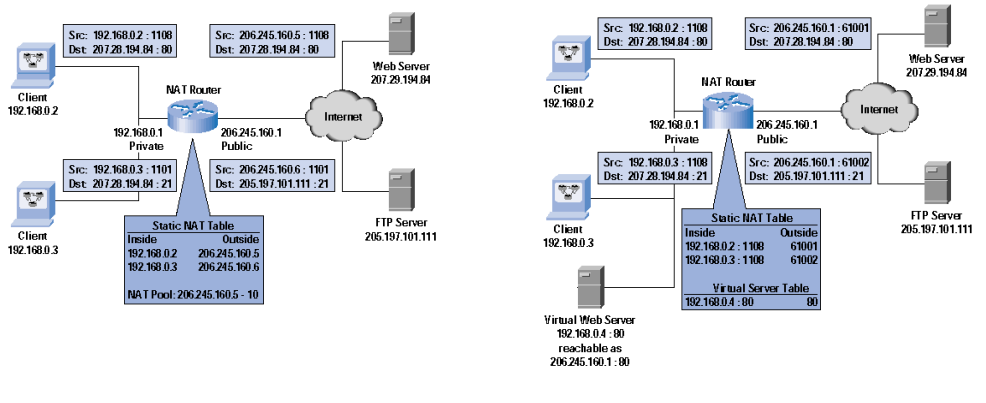
\includegraphics[scale = 0.65]{images/dynamic-NAT}
	\caption{A sinistra un esempio di NAT dinamico, a destra un esempio di NAPT.}
	\label{img:dynamic-NAT}
\end{figure}

Abbiamo detto che il server NAT svolge un \textit{mapping tra indirizzi interi ed esterni}. In generale esistono due tipi di NAT: \textit{statico} e \textit{dinamico}. Il NAT statico effettua un mapping uno-a-uno tra indirizzi esterni ed indirizzi interni: è molto facile da implementare, ma non risolve il problema della scarsità di indirizzi; per questo ha un uso molto limitato ed in genere può servire in congiunzione ad un firewall. Il NAT dinamico (Figura \ref{img:dynamic-NAT}) effettua un mapping uno-a-molti tra indirizzi esterni ed indirizzi interni; rispetto al precedente è un meno semplice da implementare e richiede un server stateful, ma risolve il problema della scarsità degli indirizzi. In questo caso può accadere però che due host interni usino la stessa porta; per ovviare a questo problema si fa ricorso al \textbf{NAPT} (\textit{Network Address and Port Translation}) (Figura \ref{img:dynamic-NAT}), che effettua un mapping dinamico tra indirizzi interni ed esterni utilizzando porte dinamiche. In sostanza i NAPT sono simili ai Network Address Translation, ai quali però viene aggiunta la funzione di tradurre anche le porte e, quindi, dare una diversa mappatura delle porte rispetto a quella vista dall'esterno. Con questa mappatura ci si riserva la possibilità di utilizzare un software anche da remoto senza aprire porte che potrebbero essere soggette ad eventuali attacchi.

Solitamente insieme al NAT viene utilizzato un altro protocollo: \textbf{IPsec} (\textit{IP security}). Sostanzialmente è uno standard che si prefigge di ottenere connessioni sicure su reti IP. La sicurezza viene raggiunta attraverso funzionalità di autenticazione, cifratura e controllo di integrità dei pacchetti IP (datagrammi); in pratica viene aggiunto un header a livello 3. IPsec è quindi una collezione di protocolli formata da alcuni che implementano lo scambio delle chiavi per realizzare il flusso crittografato ed altri che forniscono la cifratura del flusso di dati. Per quanto riguarda il secondo aspetto, esistono due protocolli: \textbf{Authentication Header (AH)} e \textbf{Encapsulating Security Payload (ESP)}. AH fornisce autenticazione e integrità del messaggio, ma non offre la confidenzialità, ESP fornisce invece autenticazione, confidenzialità e controllo di integrità del messaggio; per questi motivi ESP è molto più usato di AH. Entrambe le modalità tuttavia presentano problemi analoghi.

Problema: sia il NAT sia l'IPsec richiedono un ricalcolo dei checksum IP e TCP; le due cose possono interferire \textit{molto} male, portando ad un completo blocco delle comunicazioni.
\begin{figure}[htbp]
	\centering
	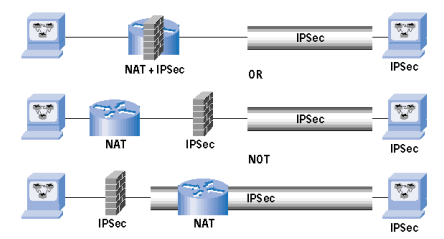
\includegraphics[scale = 0.7]{images/NAPT-IPsec}
	\caption{Possibili modi di configurazione del NAPT e IPsec.}
	\label{img:NAPT-IPsec}
\end{figure}

In Figura \ref{img:NAPT-IPsec} sono rappresentati tre diversi scenari con cui è possibile configurare NAPT e IPsec. Una idea potrebbe essere quella di porre il NAPT prima dell'IPsec (o insieme). Teoricamente queste idee sarebbero fattibili, ma non lo sono in pratica: la rete locale non viene protetta e si danno le credenziali all'IPsec. In ogni caso, un host dietro ad un NAT non può cominciare una comunicazione IPsec e la co-locazione di NAT e IPsec è un potenziale pericolo per la sicurezza. L'IPsec risulterebbe dunque un elemento di \textquotedblleft fastidio". Per ovviare al problema della comunicazione cifrata, tuttavia, potremmo scegliere due strade:
\begin{enumerate}
	\item Togliere il NAT, oppure
	\item Incapsulare il pacchetto dentro un altro pacchetto, poiché il NAT cambierà sicuramente IP e porta (non è granché come soluzione). Questa tecnica prende il nome di \textbf{IP-over-IP} o \textbf{tunneling}.
\end{enumerate}
Facciamo adesso un passo indietro ridefinendo il NAT. Il NAT nasce nel 1994 (RFC 1631) come metodo per alleviare il problema della scarsità di indirizzi IPv4; l'RFC 2776 del 2000 definisce il \textquotedblleft Network Address Translation -- Protocol Translation (NAT-PT)". L'idea di base è la seguente: in Internet i pacchetti \textquotedblleft non routable" non sono trasportati, vengono scartati dai router perché l'indirizzo IP \textit{non è univoco}; serve quindi una traslazione da indirizzo non routable ad un indirizzo routable e questo compito viene svolto dal NAT. Vediamo in dettaglio le operazioni svolte da un NAT; sostanzialmente il proprio compito è quello di effettuare un \textbf{binding}, ossia una associazione bidirezionale, in questo caso, tra triple:
$$\{\text{IP, Protocollo, Porta}\}\text{ (interna)} \Longleftrightarrow \{\text{IP, Protocollo, Porta}\}\text{ (esterna)}$$
Nella prima versione del NAT creata nel 1994 (RFC 1631) veniva variato solamente l'indirizzo IP; questa prima idea funzionava abbastanza bene, ma non risolveva la scarsità di indirizzi, poiché il numero di indirizzi necessari al NAT è pari al numero di PC che vogliono utilizzare \textit{contemporaneamente} lo stesso protocollo. Nella versione del 2000 (RFC 2776), invece, vengono variati l'indirizzo IP e la porta sorgente. Questa tecnica funziona poiché aggira il problema della scarsità di indirizzi: il numero di connessioni contemporanee (bindings) è $\approx 64000$ (well-known ports escluse).

Quando arriva un pacchetto sull'interfaccia \textit{interna} del NAT si cerca un binding: se è presente, l'header del pacchetto viene modificato e viene effettuato il forward; se invece non è presente, viene creato un binding, viene modificato l'header del pacchetto e viene effettuato il forward.

Quando arriva un pacchetto sull'interfaccia \textit{esterna} del NAT si cerca un binding: se è presente, l'header del pacchetto viene modificato e viene effettuato il forward; se invece non è presente, il pacchetto viene scartato.\\
Un binding in un server NAT viene cancellato allo scadere di un timer.

Con queste politiche un binding viene creato solamente dagli host interni che iniziano la comunicazione, poiché i pacchetti provenienti dall'esterno vengono scartati. Questo può far pensare che la rete sia sicura, ma questa concezione è del tutto sbagliata, perché se un host esterno volesse comunicare con un host interno non potrebbe farlo. A questo scopo solitamente viene introdotto anche un \textit{filter} che ha il compito di decidere quali triple esterne possono essere ritradotte nelle corrispondenti interne. Un problema dovuto all'introduzione del filter proviene dal fatto che diversi tipi di filter possono dar luogo a diversi comportamenti del NAT, cioè si potrebbe avere un comportamento non deterministico: alcuni comportamenti sono voluti, altri invece no.

Applicare NAT e filter in TCP e UDP non è la stessa cosa. Sostanzialmente in TCP è semplice perché è connection oriented, mentre in UDP è più difficile perché è connectionless; vediamo la questione più nel dettaglio.\\
In TCP, essendo un protocollo stateful, il binding è aggiornato in base a un timer che varia a seconda dello stato della connessione e della dimensione della CWIN (finestra di congestione). In UDP, essendo un protocollo stateless, il binding è basato solo su un timer e sulla \textquotedblleft conoscenza" del comportamento dell'applicazione (i.e., porte utilizzate).\\
Nel TCP il NAT ha di solito un comportamento simmetrico, ossia binding e filter sono basati sulla quintupla $\{\text{protocollo, IP sorgente, porta sorgente, IP destinazione, porta destinazione}\}$ e per effettuare il binding è sufficiente verificare il pacchetto che presenta il flag $\text{SYN} = 1$. Così facendo, le comunicazioni devono partire dall'interno e non è possibile effettuare \textit{callback}.

Tuttavia, quello che va bene per TCP non è detto che vada bene per UDP. In TCP infatti, come già detto, uno stream è definito da una quintupla ed il demultiplexing è effettuato dal kernel e definito a livello di TCP. Nell'UDP, invece, il demultiplexing viene effettuato a livello \textit{applicativo} e inoltre una singola applicazione può usare una sola socket in uscita per due stream diversi con destinatari diversi (il TCP non lo permette). Applicare NAT e filter a UDP è dunque difficile perché dovremmo sapere in anticipo cosa fa l'applicazione; idealmente questa gestione dovrebbe essere inclusa direttamente nelle applicazioni, ma la maggior parte delle software house non producono applicazioni basate su UDP di tipo \textit{NAT oriented}. Serve dunque un diverso comportamento del NAT nel caso di UDP.

Il comportamento del NAT per l'UDP è gestito in base a come viene eseguito il filter; in base a come si comporta il NAT alcuni applicativi possono o meno funzionare, in parte o del tutto. Esistono quattro diversi comportamenti:
\begin{enumerate}
	\item \textbf{Symmetric NAT}. Ogni richiesta proveniente da stesso indirizzo IP/porta e diretta ad uno specifico indirizzo IP/porta destinazione esterno è mappata in un unico indirizzo IP/porta sorgente esterno; se lo stesso host interno invia un pacchetto con lo stesso indirizzo di sorgente e di porta, ma verso un'altra destinazione, viene utilizzata una mappatura differente. Solamente l'host esterno che riceve un pacchetto da un host interno può inviare un pacchetto indietro. Non funzionano i programmi che hanno bisogno di referral \& handover (es. chat di messaggistica istantanea, MSN).
	
	\item \textbf{Full Cone NAT} (o one-to-one NAT). Una volta che un indirizzo interno (\texttt{iAddr:iPort}) viene mappato in un indirizzo esterno (\texttt{eAddr:ePort}), tutti i pacchetti provenienti da \texttt{iAddr:iPort} vengono inviati attraverso \texttt{eAddr:ePort}. Qualunque host esterno può quindi inviare pacchetti a \texttt{iAddr:iPort}, mandando pacchetti a \texttt{eAddr:ePort}. In questo caso il filter non fa nulla (è vuoto), ma chiunque può raggiungere l'host interno (può essere contattato su tutte le porte), anche i malintenzionati: è persino possibile fare un port scanning.
	
	\item \textbf{(Address)-Restricted Cone NAT}. Simile al caso precedente, ma con qualche restrizione: una volta che un indirizzo interno (\texttt{iAddr:iPort}) viene mappato in un indirizzo esterno (\texttt{eAddr:ePort}), tutti i pacchetti provenienti da \texttt{iAddr:iPort} vengono inviati attraverso \texttt{eAddr:ePort}. In questo caso, però, un host esterno \texttt{hAddr:any} può inviare pacchetti verso \texttt{iAddr:iPort} mandando pacchetti a \texttt{eAddr:ePort} solo se \texttt{iAddr:iPort} ha inviato in precedenza un pacchetto a \texttt{hAddr:any} (in questo caso \texttt{any} significa che il numero di porta non è rilevante). In questo caso quindi il filter è basato sull'indirizzo IP del destinatario; questa scelta è limitante, chat di messaggistica istantanea o programmi P2P ad esempio non funzionano.
	
	\item \textbf{Port Restricted Cone NAT}. Questo caso è simile ad un Address Restricted Cone NAT, ma le restrizioni includono i numeri di porta: una volta che un indirizzo interno (\texttt{iAddr:iPort}) viene mappato in un indirizzo esterno (\texttt{eAddr:ePort}), tutti i pacchetti provenienti da \texttt{iAddr:iPort} vengono inviati attraverso \texttt{eAddr:ePort}. In questo caso, un host esterno \texttt{hAddr:hPort} può inviare pacchetti verso \texttt{iAddr:iPort} mandando pacchetti a \texttt{eAddr:ePort} solo se \texttt{iAddr:iPort} ha inviato in precedenza un pacchetto a \texttt{hAddr:hPort}. In questo caso quindi il filter è basato anche sulla \textit{porta} del destinatario; in questa situazione funzionano quasi tutti i programmi UDP, anche se con delle limitazioni.
\end{enumerate}
Come fare se volessimo raggiungere un host appartenente alla stessa rete? Una prima idea, non tanto intelligente, potrebbe essere quella di far uscire e rientrare il pacchetto attraverso il NAT. Un'idea più furba è l'\textbf{hairpin} e può comportare o meno l'uso di indirizzi esterni. L'hairpinning (o NAT loopback) descrive una comunicazione tra due host che stanno dietro allo stesso dispositivo NAT utilizzando la propria mappa di endpoint. Poiché non tutti i dispositivi NAT supportano questa configurazione di comunicazione, le applicazioni dovrebbero esserne a conoscenza.
\begin{figure}[htbp]
	\centering
	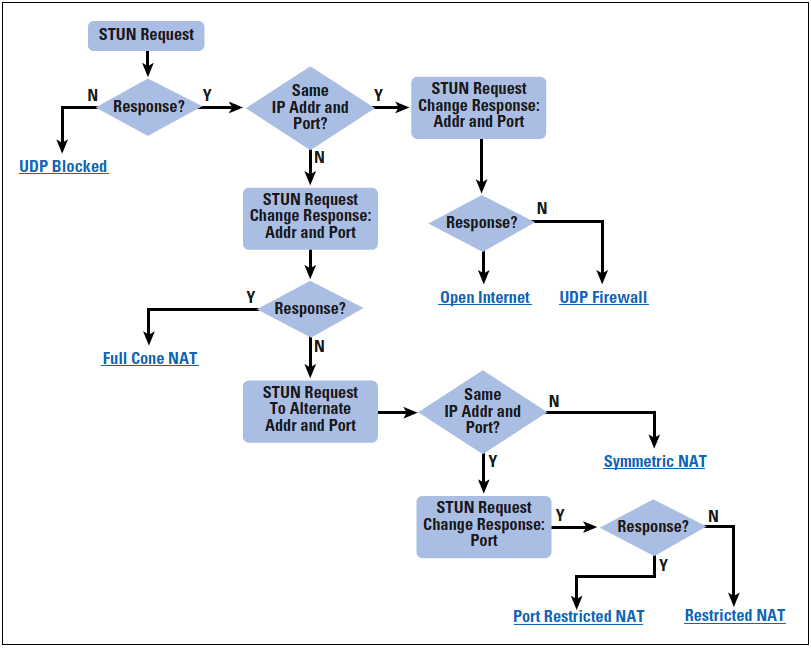
\includegraphics[scale = 0.4]{images/STUN}
	\caption{STUN Diagram (RFC 3489).}
	\label{img:STUN}
\end{figure}

Affinché un host possa sapere quale tipo di NAT viene usato in una rete è necessario un protocollo in grado di rivelarlo. Introduciamo pertanto lo \textbf{STUN} (RFC 3489), un protocollo tipo request-reply (o try\&error) in grado di scoprire il tipo di NAT in uso. In Figura \ref{img:STUN} è riportato il diagramma dell'algoritmo generale utilizzato dallo STUN.

Si noti, come già detto, che il NAT può essere \textit{non deterministico}, ossia potrebbe cambiare il proprio comportamento a seconda della disponibilità delle risorse. O, ancora, potrebbero esserci più NAT nel path sorgente/destinazione: in tal caso la classificazione non è rigorosa ed il comportamento non è prevedibile; il secondo livello di NAT potrebbe avere lo stesso comportamento del primo. Dunque lo STUN \textquotedblleft fotografa" il comportamento del NAT ad un certo istante temporale, ma questo può variare sulla base delle risorse a disposizione, quindi del carico.\\
Vediamo adesso una classificazione più precisa del binding, ossia di come può lavorare un server NAT:
\begin{itemize}
	\item \textbf{Endpoint independent}. Il NAT riusa il binding per tutte le sessioni provenienti dallo stesso IP/porta, l'IP/porta esterno non è valutato; è come un \textit{Full Cone NAT}.
	
	\item \textbf{Endpoint address dependent}. Il NAT riusa il binding per tutte le sessioni provenienti dalla stesso IP/porta verso lo stesso IP esterno (la porta non si considera); è come un \textit{Restricted Cone NAT}.
	
	\item \textbf{Endpoint address and port dependent}. Si utilizza la quintupla $$\{\text{protocollo, IP sorgente, porta sorgente, IP destinazione, porta destinazione}\},$$ cioè si riutilizza lo stesso mapping per tutti i pacchetti inviati ai medesimi IP/porta esterni; è come un \textit{Symmetric NAT}.
	
	\item \textbf{Endpoint port dependent}. Il NAT riusa il binding per tutte le sessioni provenienti dalla stesso IP/porta verso la stessa porta esterna (l'IP non si considera); è come un \textit{Port Restricted Cone NAT}.
\end{itemize}
Il port binding lo possiamo suddividere in tre categorie:
\begin{itemize}
	\item \textbf{Port preservation}. Il NAT può tentare di mantenere la porta di origine. Nel caso in cui due host interni abbiano la stessa porta di origine, ad uno sarà cambiata la porta, mentre all'altro no.
	
	\item \textbf{Port overloading}. Il NAT fa una sorta di port preservation in modo aggressivo; in questo caso un secondo tentativo di binding fa scadere il binding esistente, dunque la porta non viene cambiato all'ultimo host che fa richiesta.
	
	\item \textbf{Port multiplexing}. Il NAT si occupa di fare demultiplexing cercando di mandare tutte le comunicazioni su una porta. All'esterno i pacchetti appaiono come se provenissero dallo stesso IP/porta, il NAT si occuperà di effettuare il demultiplexing corretto. Tuttavia, se due host interni volessero mandare due stream allo stesso host/porta esterno, allora non sarebbe possibile il demultiplexing. In questo caso uno dei due stream avrebbe assegnata una porta diversa. È dunque un \textit{comportamento non deterministico} in casi di traffico elevato.
\end{itemize}
Per il timer abbiamo quattro politiche di aggiornamento:
\begin{itemize}
	\item \textbf{Bidirectional}. Il timer viene aggiornato dai pacchetti che transitano in entrambi i sensi.
	\item \textbf{Outbound}. Il timer viene aggiornato solo dai pacchetti che transitano dall'interno verso l'esterno. L'aspetto negativo è che l'host interno deve rinnovarlo periodicamente, poiché se quest'ultimo riceve solamente il timer scade; è necessario dunque utilizzare un \textit{keep-alive}. Inoltre il timer potrebbe essere per-session o per-binding, nel caso di riuso del binding per più sessioni.
	\item \textbf{Inbound}. Il timer viene aggiornato solo dai pacchetti che transitano dall'esterno verso l'interno. Anche in questo caso è necessario un keep-alive.
	\item \textbf{Transport Protocol State}. Si effettua un'inferenza del tempo di vita/timing basandosi su informazioni di livello trasporto. All'atto pratico risulta molto difficile da programmare ed eventuali bug potrebbero dar luogo a vulnerabilità utilizzabili per attacchi di tipo DoS. Il problema è simile a quello del layer 7 del firewall (L7 filtering).
\end{itemize}
Vediamo, infine, una classificazione precisa per il filtering esterno:
\begin{itemize}
	\item \textbf{Endpoint independent}. Il filter non filtra o scarta i pacchetti: è come un \textit{Full Cone NAT}.
	
	\item \textbf{Endpoint address dependent}. Il filter filtra i pacchetti che non provengono dall'IP destinatario del binding: è come un \textit{Restricted Cone NAT}.
	
	\item \textbf{Endpoint address and port dependent}. Il filter filtra i pacchetti che non provengono dall'IP/porta destinatario del binding: è come un \textit{Symmetric NAT} od un \textit{Port Restricted Cone NAT}.
\end{itemize}
Si noti che il filter potrebbe avere un timer separato simile a quello del binding (i timer possono essere in qualche modo correlati).

\subsubsection{Considerazioni}
\begin{itemize}
	\item Le applicazioni P2P tentano di aggirare i NAT, ma così facendo si creano spesso problemi di sicurezza; \textquotedblleft bucare" in questo caso può significare aprire un numero di porte arbitrario.
	\item Protocolli simili a ICMP rischiano di fallire, perché nei payload sono spesso contenute informazioni relative all'IP/porta sorgente. Inoltre vi è la necessità di calcolare i checksum e molti NAT non supportano questo tipo di funzionalità, dunque molti pacchetti vengono scartati poiché i checksum non risultano validi.
	\item Il processo di IP fragmentation prevede di ricostruire i pacchetti (o mantenere informazioni del primo frammento), perché nei frammenti successivi l'header TCP/UDP è assente, ma questo potrebbe portare ad un attacco a frammentazione (si consideri anche che il primo frammento potrebbe arrivare fuori sequenza). Inoltre, genericamente il NAT attende l'arrivo di tutti i frammenti e nel caso in cui questi non siano stati ricevuti entro un tempo prestabilito, quelli in memoria vengono scartati: questo potrebbe comportare un grande spreco di risorse.
\end{itemize}
Altri protocolli potrebbero avere gli stessi tipi di problemi ed il NAT può tentare di modificare il contenuto stesso del payload. Esistono però dei protocolli che mirano a concordare automaticamente le tecnologie che si vogliono utilizzare (e.g. tipo di NAT) ed altre opzioni di comunicazione (e.g. tempo dopo il quale dei pacchetti vengono scartati):
\begin{itemize}
	\item \textbf{Universal Plug and Play (UPnP)}. È un insieme di protocolli e procedure per la definizione e l'annuncio di device e servizi. \textquotedblleft\textit{A UPnP compatible device from any vendor can dynamically join a network, obtain an IP address, announce its name, convey its capabilities upon request, and learn about the presence and capabilities of other devices.}" [Wikipedia]
	\item \textbf{Internet Gateway Device (IGD) Standardized Device Control Protocol}. Permette ad un device UPnP di scoprire l'indirizzo esterno di un NAT e di creare binding/filters per i suoi servizi in maniera automatica.
\end{itemize}
L'aspetto positivo di questo tipo di protocolli è che tutto funziona molto bene ed in modo automatico, quello negativo è che le porte del NAT sono aperte in maniera incontrollata e potrebbero sovrascrivere dei binding esistenti (come ad esempio per la porta 80).